\section{System Demonstration}
\label{sec-demo}

\begin{figure*}[tp]
\centering
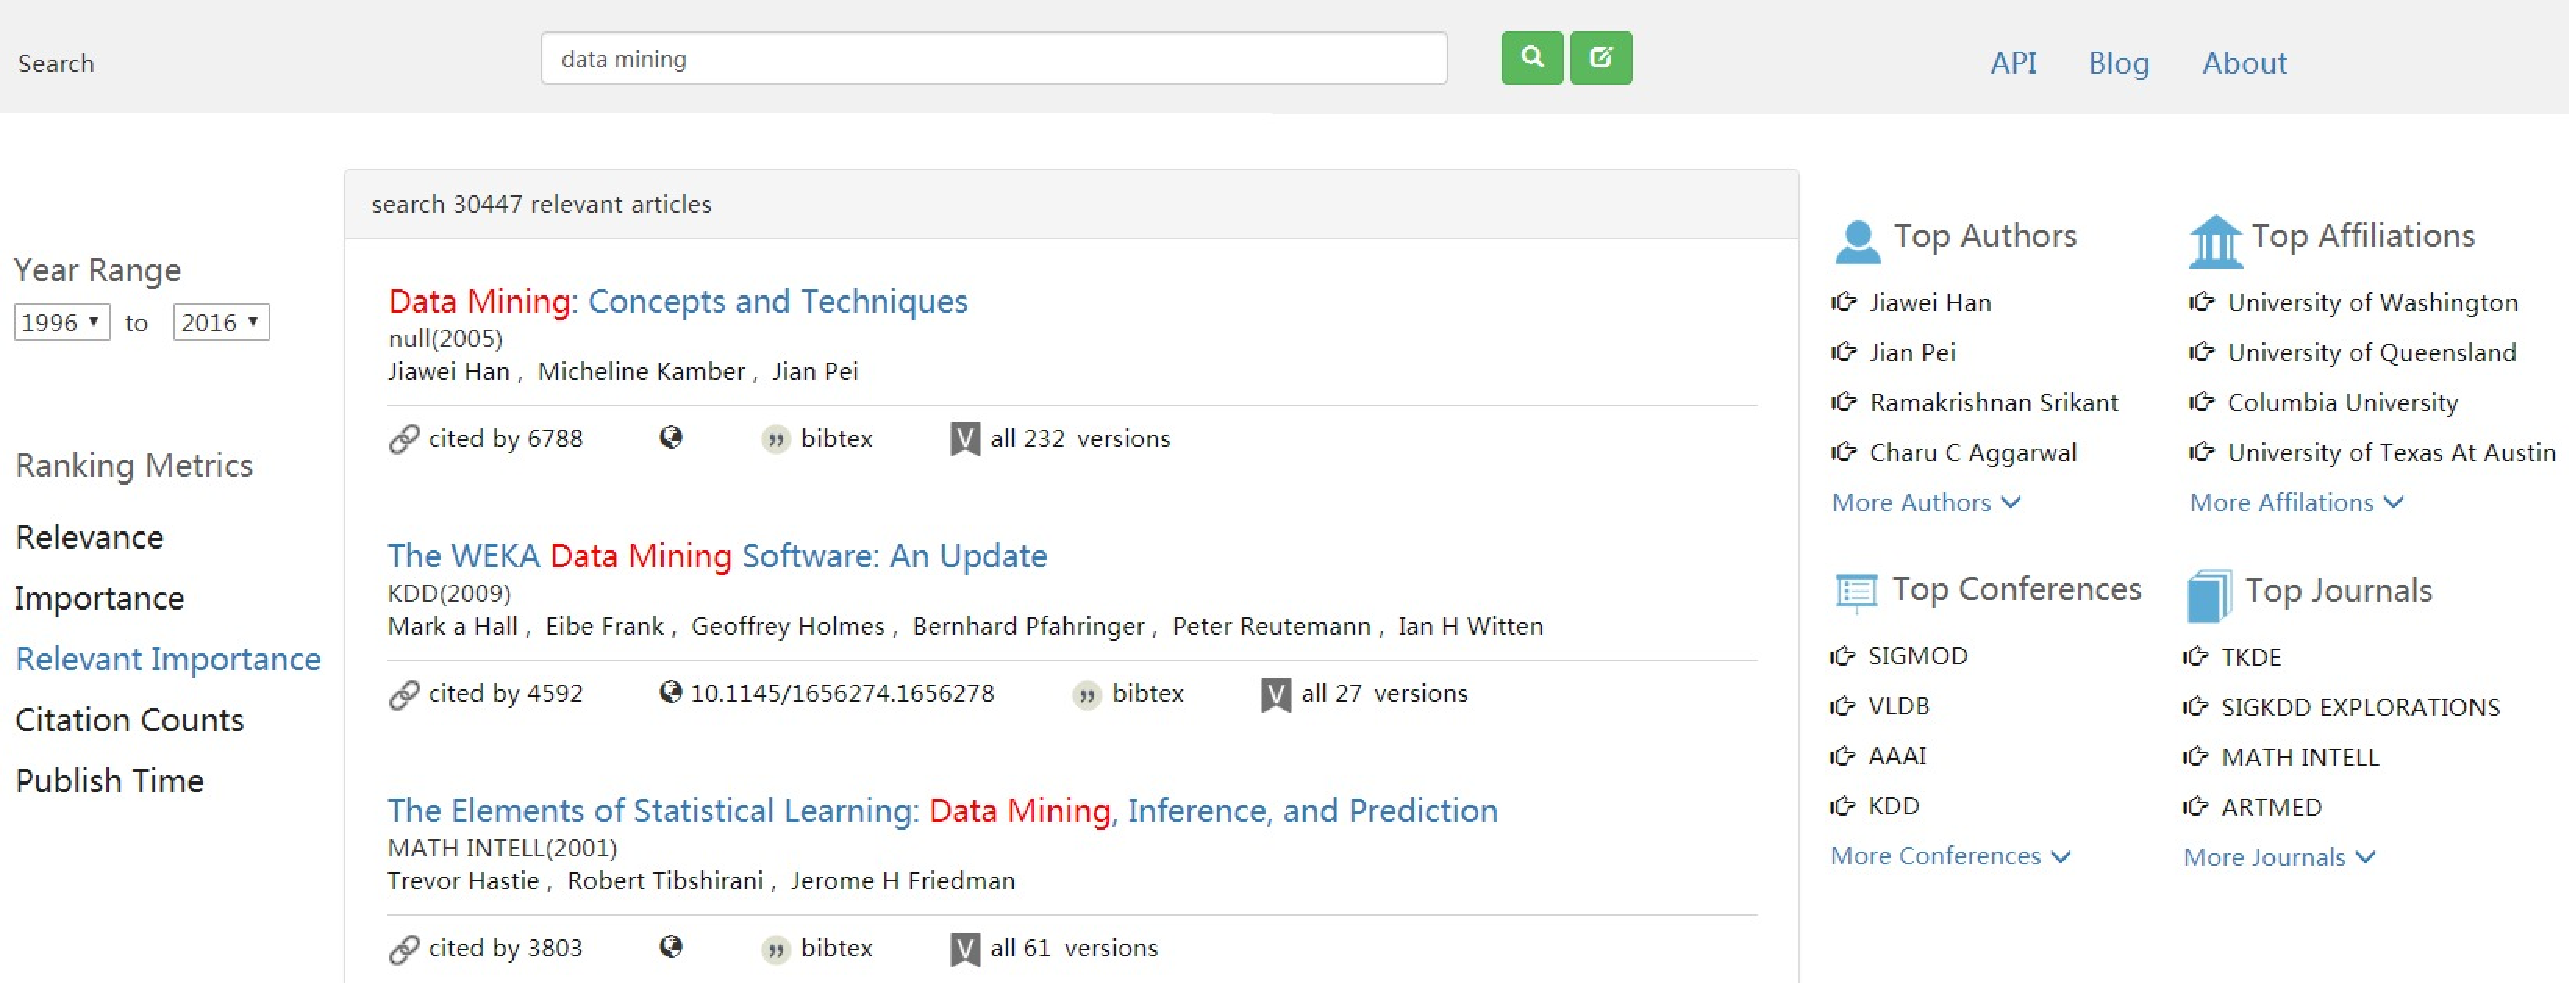
\includegraphics[width=\textwidth]{searchKeywords.pdf}
\vspace{-3ex}
\caption{Demonstration of heterogeneous entity ranking}
\label{fig:searchKeywords}
%\vspace{-2ex}
\end{figure*}

\begin{figure}
\centering
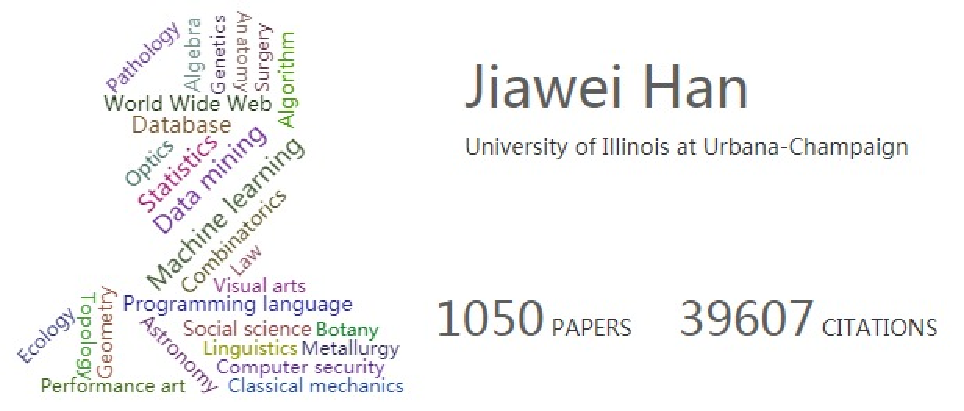
\includegraphics[width=\columnwidth]{hjwAvatar.pdf}
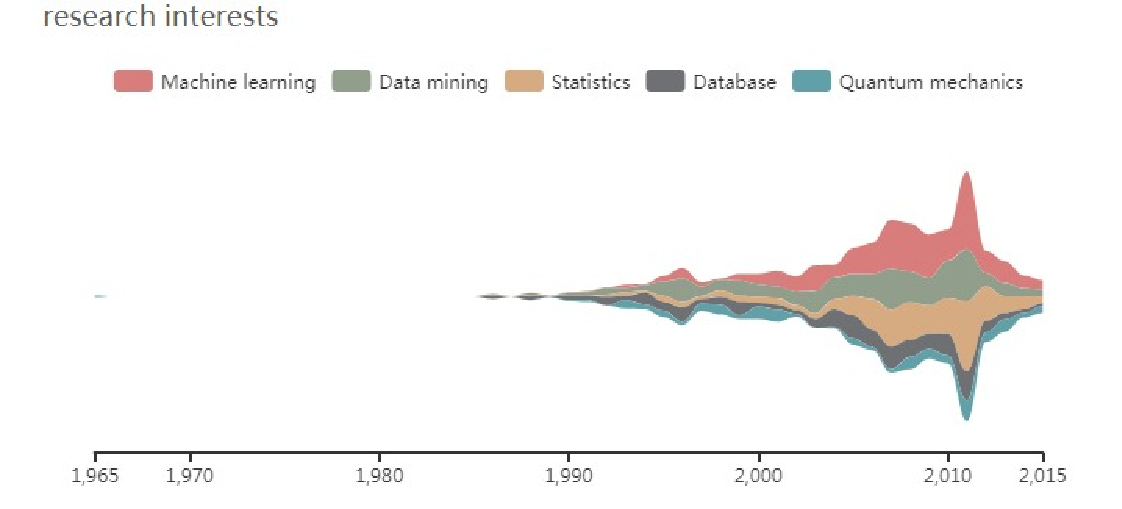
\includegraphics[width=\columnwidth]{hjwInterest.pdf}
%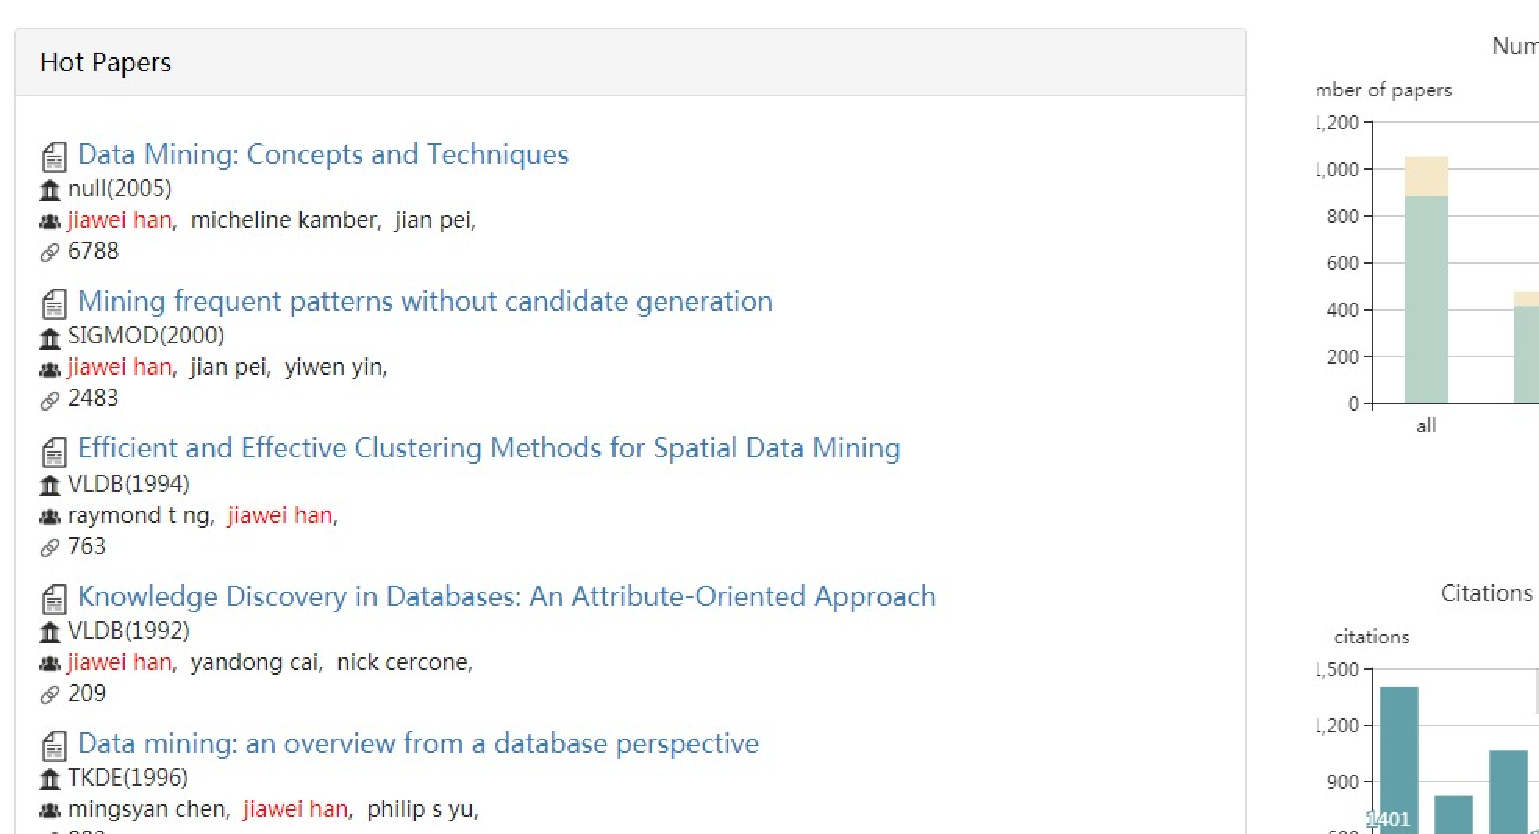
\includegraphics[width=\columnwidth]{hjwPapers.pdf}
\vspace{-2ex}
\caption{Demonstration of author profiling}
\label{fig:hjwProfile}
%\vspace{-2ex}
\end{figure}

The demonstrate our system from three aspects: (i) heterogeneous entity ranking, (ii) author profiling, and (iii) performance comparison between Neo4j and RDBMS MySQL.


%The demonstration consists of three parts. (1) We walk through its various ranking metrics to demonstrate the ability of \oursystem to query and rank heterogeneous entities. (2) To further illustrate the profiling function based on scholarly data analysis, we take author profiling as an example. (3) In the scholarly information search scenario, we compare the query performance of MySQL and Neo4j through experiments.

\stitle{Heterogeneous entity ranking}.
Figure~\ref{fig:searchKeywords} presents the heterogeneous entity rankings under query ``graph database".
%
The ranking metrics are displayed in the left. Note that \oursystem also supports querying articles and other entities within a specific range of year.
When sorting by relevant importance, the rankings of articles and other entities, \ie authors, affiliations, journals and conferences, are shown in the middle and right side.
%For instance, Dr. Lei Chen, Mihalis Yannakakis, Jeffrey Xu Yu, M Tamer Ozsu are ranked as top authors in the field of graph database.
%
Finally, it is worth pointing out that users can also directly query entities by typing their names in the search box on top. %in \oursystem.




\stitle{Author profiling}.
Figure~\ref{fig:hjwProfile} gives an example of author profiling for Prof. Jiawei Han.
Basically, the affiliation and numbers of published papers and citations are presented.
Moreover, the word cloud gives a summary description of the author's fields of study, where the size of words represents its importance in the author's research career. For instance, data mining and machine learning are identified as Prof. Jiawei Han's most important fields of study.
Moreover, \oursystem details the evolution of research interest, shown in the bottom of Fig.~\ref{fig:hjwProfile}. %by counting the numbers of publications in the top fields of study.
%His publications keep growing before 2010, and the convex near 2011 is due to his numerous and influential publications such as ``data mining: concepts and techniques".
Besides, users can also find the relevant articles in each field of study. Other functions in author profiling include co-author analysis and statistics by time. We omit the demonstration of those functions due to space limitation.


\stitle{Performance comparison: Neo4j vs. MySQL}.
Lastly, we compare the query performance of the adopted graph database Neo4j with traditional RDBMS MySQL. More specifically, we consider three types of queries, \ie (i) finding the title and authors of a paper given paper ID, (ii) finding the top-10 most important citations of a paper given paper ID, and (iii) finding the top-10 most important papers published by an author given author ID.
Note that the numbers of joins are (2, 3, 4) for the three types of queries in MySQL, respectively. As people care more about those ``good'' papers, we thus randomly selected 1000 papers/authors whose numbers of citations/published-articles are no less than 100/50, respectively, and computed the average processing time, shown in Table~\ref{tab-compare}.
% 14.8%	19.4 %	45.3%
As can be seen, Neo4j is consistently more efficient than MySQL, which is on average (14.8\%, 19.4\%, 45.3\%) faster for the three types of queries.
Thus, structure-aware Neo4j is more efficient than MySQL for scholarly analysis, especially for complex queries with more join operations.


\begin{table}[t!]
\begin{center}
\caption{Query performance comparison: Neo4j vs. MySQL}
\vspace{-1ex}
\label{tab-compare}
\begin{scriptsize}
\begin{tabular}{c c c c} %{lp{2cm}p{2cm}p{2cm}}
\hline
{} & {Type 1 queries} & {Type 2 queries} & {Type 3 queries}\\
\hline
MySQL & 0.115 sec.  & 2.89 sec. & 3.60 sec. \\
Neo4j & 0.098 sec.  & 2.33 sec. & 1.97 sec. \\
\hline
\end{tabular}
\end{scriptsize}
\vspace{-3ex}
\end{center}
\end{table}


\eat{
\stitle{Ranking Instance} We rank the conference papers \eg SIGMOD following the metrics of {\em time ranking}. We only collect articles published earlier than 2016, so the top of {\em time ranking} is the maximum importance score in 2015. As shown in fig. \ref{fig:sigmod}, we put ``Spark SQL: Relational Data Processing in Spark" in second place, which has the most citations(653) in SIGMOD 2015 up to now. More generally, in our top 10, there are 3 articles that has the most citation in SIGMOD 2015.
% the description in ICDE 2018

\par
Although they share the same venue component in the same year, the author of the article has higher prestige and popularity, such as Matei Zaharia and Michael Armbrust. Besides, an article in VLDB cites the paper published in the same years that increases the prestige and popularity of the citation components. Thus, the paper possesses a higher importance score by assembling the component of citation, author and venue.
}

%\par
%\stitle{Affiliation profiling}. As shown in fig. \ref{}, we give an example of affiliation profiling. The layout of the Affiliation Page is similar with Search Page, users can discover publications using various ranking metrics and check statistics information, such as the importance author, relevant affiliation, famous journals/conferences.
%% affiliation profiling
%\par
%\stitle{Venue profiling} venue
